%%%%%%%%%%%%%% main.tex %%%%%%%%%%%%%%%%
%% Archivo principal de templateLatex %%
%% usado para construir el pdf.       %%
%%%%%%%%%%%%%%%%%%%%%%%%%%%%%%%%%%%%%%%%
% Por marcosgatica2003
% Link del repositorio: https://github.com/marcosgatica2003/gaticonStandards

\documentclass[a4paper]{article}

\input{packages}
\input{comandos}

\begin{document}
    \input{caratula}
    \input{fancyConfig}
    \input{indiceConfig}
    \pagestyle{fancy}
    \newpage
\section{Polarización del punto Q}
\sangria{En este trabajo implementamos un transistor JFET en configuración fuente común, para aplicar el modelo MES, en esta oportunidad implementamos el modelo con autopolarización. Nuestros datos iniciales fueron $V_{DD}= 12V$ $R_G=1M\Omega$, además contabamos también con los datos del punto Q ya predefinidos $I_{DQ}=\frac{I_{DSS}}{2}$ y $V_{DSQ}=\frac{V_{DD}}{2}$}
\sangria{Primero revelamos la curva de $I_{DSS}$, para luego calcular $R_S$ $R_D$, la curva relevada fue la siguiente.}
\midTitle{blue}{Mediciones de $I_{DSS}$ Obtenidas}{}
\begin{center}
\setlength{\tabcolsep}{4pt}
\captionof{table}{Mediciones de $I_{DSS}$ en función de $V_{DS}$.}
\begin{tabular}{|
>{\columncolor[HTML]{FFCCC9}}c |
c | c |}
\hline
\rowcolor[HTML]{FFFFC7}
\textbf{$V_{DS}$ (V)} & \textbf{$I_{DSS}$ (mA)} & \textbf{Diferencia (\%)} \\ \hline
0.200 & 2.112 & - \\ \hline
0.440 & 4.530 & 114.5 \\ \hline
0.600 & 5.500 & 21.4 \\ \hline
0.820 & 6.050 & 10.0 \\ \hline
1.015 & 6.390 & 5.6 \\ \hline
1.235 & 6.560 & 2.7 \\ \hline
1.402 & 6.650 & 1.4 \\ \hline
1.650 & 6.742 & 1.4 \\ \hline
1.815 & 6.787 & 0.7 \\ \hline
2.020 & 6.834 & 0.7 \\ \hline
2.200 & 6.853 & 0.3 \\ \hline
2.450 & 6.893 & 0.6 \\ \hline
2.609 & 6.913 & 0.3 \\ \hline
2.830 & 6.942 & 0.4 \\ \hline
\end{tabular}
\end{center}

\begin{figure}[H]
    \centering
    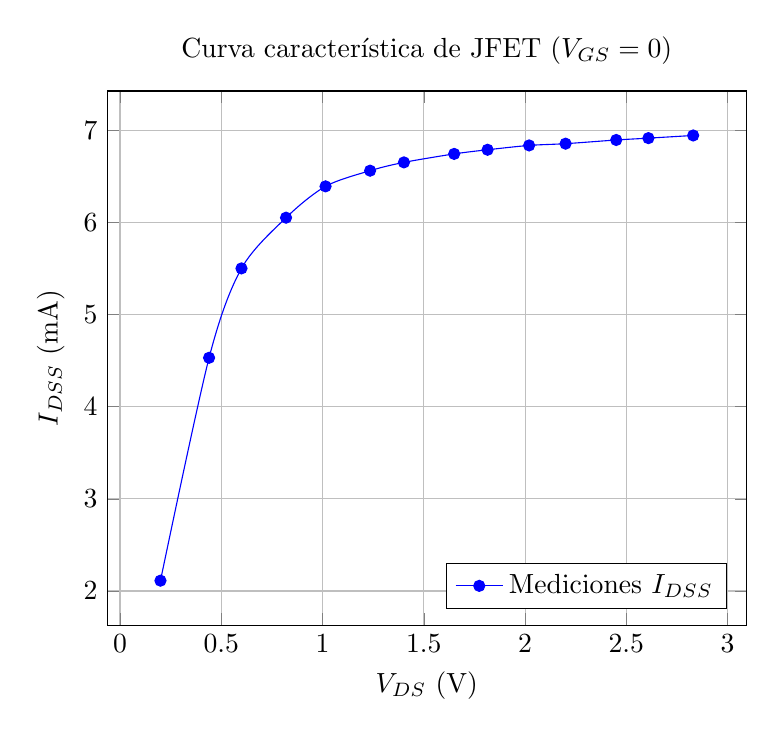
\begin{tikzpicture}
    \begin{axis}[
        title={Curva característica de JFET ($V_{GS} = 0$)}, % Título del gráfico
        xlabel={$V_{DS}$ (V)},          % Etiqueta eje X
        ylabel={$I_{DSS}$ (mA)},        % Etiqueta eje Y
        grid=major,                   % Grilla principal
        legend pos=south east,        % Posición de la leyenda (esquina inf. derecha)
        width=0.8\textwidth,          % Ancho del gráfico
    ]

    \addplot [
        smooth,     % Suaviza la línea que une los puntos
        mark=*,     % Pone un marcador en cada punto de la tabla
        blue,       % Color de la línea
    ]
    % Aquí van los datos Vds (x) e Idss (y) de tu tabla
    coordinates {
        (0.200, 2.112)
        (0.440, 4.530)
        (0.600, 5.500)
        (0.820, 6.050)
        (1.015, 6.390)
        (1.235, 6.560)
        (1.402, 6.650)
        (1.650, 6.742)
        (1.815, 6.787)
        (2.020, 6.834)
        (2.200, 6.853)
        (2.450, 6.893)
        (2.609, 6.913)
        (2.830, 6.942)
    };
    \addlegendentry{Mediciones $I_{DSS}$}

    \end{axis}
    \end{tikzpicture}
    \caption{Curva de salida $I_D = f(V_{DS})$ para $V_{GS} = 0$.}
    \label{fig:curva_jfet}
\end{figure}
\newpage
\subsubsection{Cálculos del punto Q}
\sangria{Una vez revelada la curva, el valor de $I_{DSS}$ se extrajo a partir de las diferencias porcentules del mismo valor, el valor elejido fue: $I_{DSS} = 6,650mA$, ya que la diferencia porcentual con el valor anterior fue del $1.4\%$, el valor de tensión en este punto se denomina $V_{GSoff}$ y es de $V_{GSoff}=1,402V$}

$$I_{DQ}=\frac{I_{DSS}}{2}$$
$$I_{DQ}=\frac{6,650mA}{2}$$
$$I_{Q}=3,325mA$$

\sangria{El siguiente paso fue calcular las resistencias para situar el punto Q, para esto primero obtenemos el valor de $V_{GS}$ para luego obtener $R_S$ y finalmente obtenemos $R_D$. Las ecuaciones de las cuales obtenemos estos valores son las siguiente:}

$$i_{D}=I_{DSS}*(1-\frac{V_{GS}}{V_{GSoff}})^2$$
$$V_{GS}=-i_{D}*R_{S}$$
$$V_{DD}=i_{D}*(R_{S} + R_{D})+V_{DS}$$

\sangria{De la primera ecuación despejamos $V_{GS}$, como nos encontramos en el punto Q, podemos sustituir $i_D$ por $I_{DQ}$ y queda:}
$$V_{GS}=(\sqrt{\frac{i_D}{I_{DSS}}}-1)*-V_{GSoff}$$
$$V_{GS}=(\sqrt{\frac{I_{DQ}}{I_{DSS}}}-1)*-V_{GSoff}$$
$$V_{GS}=(\sqrt{\frac{I_{DSS}}{2*I_{DSS}}}-1)*-V_{GSoff}$$
$$V_{GS}=(\sqrt{\frac{1}{2}}-1)*-V_{GSoff}$$
$$V_{GS}=-0,4106V$$

\sangria{Con este dato podemos obtener $R_S$ a partir de la segunda ecuación:}
$$R_S={\large{|}\frac{-V_{GS}}{I_{DQ}}}\large{|}$$
$$R_S=123,48\Omega$$
\sangria{Ya con este valor podemos calcular $R_D$}
$$$$

<<<<<<< Updated upstream
%     \section{Mediciones de pequeña señal }
\imagen[Modelo híbrido de pequeña señal]{15cm}{./imagenes/pequena.png}
\sangria{} Para el análisis de pequeña señal, se utiliza el modelo híbrido de pequeña señal del JFET. Donde la impedancia de entrada es igual al valor de la resistencia $Z_i=R_G$. La impedancia de salida es la resistencia $r_{ds}$ en paralelo con la resistencia de drenaje $R_D$.
\sangria{} Como el valor de $r_{ds}$ es muy grande, se puede despreciar su efecto en el circuito. Por lo tanto, la impedancia de salida queda $Z_o \approx R_D$.
\sangria{} Por lo tanto:
\begin{equation*}
    Z_i = R_G = \SI{1}{\mega\ohm}
\end{equation*}
\begin{equation*}
    Z_o \approx R_D = \SI{1681,51}{\ohm}
\end{equation*}
\sangria{} La ganancia de tensión se calcula como:
\begin{equation*}
    A_v = -g_m \cdot R_D
\end{equation*}
\begin{equation*}
    A_v = -(-\frac{2I_{DSS}}{V_{GSoff}})(1-\frac{V_{GSQ}}{V_{GSoff}}) \cdot R_D
\end{equation*}
\begin{equation*}
        A_v = -(-\frac{2(6.25mA)}{1,402V})(1-\frac{6V}{1,402V}) \cdot \SI{1681,51}{\ohm}
\end{equation*}
\begin{equation*}
        A_v = 52,314
\end{equation*}
\sangria{} Por lo tanto, la ganancia de corriente es:
\begin{equation*}
    A_i = -g_m \cdot R_G
\end{equation*} 
\begin{equation*}
    A_i = -(-\frac{2I_{DSS}}{V_{GSoff}})(1-\frac{V_{GSQ}}{V_{GSoff}}) \cdot R_G 
\end{equation*}
\begin{equation*}
        A_i = -(-\frac{2(6.25mA)}{1,402V})(1-\frac{6V}{1,402V}) \cdot \SI{1}{\mega\ohm}
\end{equation*}
\begin{equation*}
        A_i = 31111
\end{equation*}
\subsection{Calculo experimental de ganancia de tensión, corriente e impedancia de entrada}
\imagen[Circuito para realizar las mediciones de pequeña señal]{15cm}{./imagenes/lala.png}
\sangria{} Para hacer las mediciones de la impedancia de entrada, ganancia de tensión y ganancia de corriente se inserta la señal de $1kHz$ por el capacitor de acoplamiento en la base del transistor $C_i$ y se va aumentando la tensión de la señal de entrada hasta tener una tensión de salida de $V_L=1V_{pp}$, $V_L$ se mide la rama del drenador y $R_D$.
\sangria{} Para hacer estas mediciones se se agrega una resistencia en serie en la entrada de la base denominada resistencia sensora $R_S=1M\Omega$ que es igual a $Z_i$ calculado anteriormente.En este resistor se mide la tensión $V_g$ y $V_i$.
\sangria{}
\sangria{} La impedancia de entrada se calcula como:
\begin{center}
    \Large
    \[ Z_i=\frac{V_i}{I_i}=\frac{V_i}{\frac{V_g-V_i}{R_S}} \]
    \normalsize %
\end{center}
\sangria{} La ganancia de corriente se calcula como:
\begin{center}
    \Large
    \[ A_i=\frac{i_L}{i_i}=\frac{V_L/R_L}{(V_g-V_i)/R_S} \]
    \normalsize %
\end{center}
\sangria{} La ganancia de tensión se calcula como:
\begin{center}
    \Large
    \[ A_v=\frac{V_L}{V_i} \]
    \normalsize %
\end{center}
\midTitle{blue}{Mediciones Obtenidas}{}
\begin{itemize}
    \item $V_L=1V_{pp}$
    \item $V_i=37mV_{pp}$
    \item $V_g=71mV_{pp}$
    \item $R_S=1M\Omega$
    \item $R_L=R_D=1800\Omega$
\end{itemize}
\sangria{} Con los valores obtenidos en las mediciones se tienen los siguientes resultados:  
\begin{center}
    \Large
    \[ Z_i=\frac{3,7mV}{\frac{71mV-37mV}{1M\Omega}}=1,088M\Omega \]
    \normalsize %
\end{center}
\begin{center}
    \Large
    \[ A_i=\frac{1V/1800\Omega}{(71mV-37mV)/1M\Omega}=16,339K \]
    \normalsize %
\end{center}
\begin{center}
    \Large
    \[ A_v=\frac{V_L}{V_i}=\frac{1V}{37mV}=27,027 \]
    \normalsize %
\end{center}
%     \subsection{Cálculo experimental de impedancia de salida}

\imagen[Circuito para medir impedancia de salida]{15cm}{./imagenes/pepe.png}

\sangria{Para medir la impedancia de salida se pasiva la fuente de señal de entrada ($V_i=0$) y se conecta una resistencia sensora ($R_{sensor} = \SI{1.8}{\kilo\ohm}$) en serie con el capacitor de acoplamiento. Se inserta una señal de $1\text{ kHz}$ por esta rama y se mide la tensión $V_g$ (antes de la $R_{sensor}$) y $V_o$ (en el drenador), buscando ajustar $V_o=1\text{ V}_{pp}$.}

\sangria{La impedancia de salida se calcula como:}
$$Z_o=\frac{V_o}{I_o}=\frac{V_o}{\frac{V_g-V_o}{R_{sensor}}}$$

\midTitle{blue}{Mediciones Obtenidas (Zo)}{}
\begin{itemize}
    \item $V_o=1\text{ V}_{pp}$
    \item $V_g=2,25\text{ V}_{pp}$
    \item $R_{sensor}=\SI{1.8}{\kilo\ohm}$
\end{itemize}

\sangria{Con los valores obtenidos en las mediciones se tiene el siguiente resultado:}
$$Z_o=\frac{1\text{ V}}{\frac{2,25\text{ V}-1\text{ V}}{1800\ \Omega}} \quad \rightarrow \quad Z_o = 1440\ \Omega$$

\sangria{Con este valor de impedancia de salida se puede calcular el valor de $r_{ds}$ del transistor:}
$$Z_o=r_{ds} \parallel R_D \quad \rightarrow \quad r_{ds}=\frac{Z_o \cdot R_D}{R_D-Z_o}$$
\sangria{Usamos el $R_D$ normalizado ($1.8\text{ k}\Omega$) y el $Z_o$ medido:}
$$r_{ds}=\frac{1440\ \Omega \cdot 1800\ \Omega}{1800\ \Omega-1440\ \Omega} \quad \rightarrow \quad r_{ds} = 7200\ \Omega$$

% --- TABLA COMPARATIVA FINAL ---
\begin{table}[H]
\caption{Comparativa de parámetros de Pequeña Señal (Calculado vs. Medido)}
\label{tab:comparativa-ac-final} % ¡Recordá usar un label único!
\resizebox{\textwidth}{!}{%
\begin{tabular}{|
>{\columncolor[HTML]{FFCCC9}}c |
c | c | c |}
\hline
\rowcolor[HTML]{FFFC9E}
\textbf{Parámetro} & \textbf{Valor Calculado (Analítico)} & \textbf{Valor Medido (Experimental)} & \textbf{Desvío Porcentual} \\ \hline

% Fila Zi
$Z_i$ & $\SI{1}{\mega\ohm}$ & $1,088\text{ M}\Omega$ & 8,8\% \\ \hline

% Fila Zo
$Z_o$ & $1681,51\ \Omega$ & $1440\ \Omega$ & 14,4\% \\ \hline

% Fila Av
$A_v$ & $20,62$ & $27,027$ & 31,1\% \\ \hline

% Fila Ai
$A_i$ & $12263$ & $16339$ & 33,2\% \\ \hline
\end{tabular}%
}
\end{table}

% --- SECCIÓN DE RESULTADOS ---
\midTitle{teal}{Resultados}{}

\sangria{Las mediciones experimentales de pequeña señal muestran una excelente correlación en la impedancia de entrada $Z_i$, con un desvío de solo \textbf{8.8\%} respecto al valor teórico de $\SI{1}{\mega\ohm}$. La impedancia de salida $Z_o$ también arrojó un valor ($1440\ \Omega$) cercano al esperado ($1681,51\ \Omega$), con un desvío del \textbf{14.4\%}. Esto nos permitió estimar la resistencia interna del JFET, $r_{ds}$, en $7.2\text{ k}\Omega$.}

\sangria{Las ganancias de tensión y corriente presentaron un desvío mayor ($31,1\%$ y $33,2\%$ respectivamente). Esto es esperable, ya que la ganancia depende directamente de $g_m$, un parámetro que varía significativamente con el punto Q real del circuito (el cual se ajustó con $R_S=80,2\ \Omega$ en la práctica) y con las características propias del transistor utilizado.}

     % \newpage
\section{Polarización Con fuente de corriente}
\subsection{Cálculo de $R_1$}
\midTitle{red}{Parte analítica}{}
\sangria{En la segunda parte del trabajo práctico, se reemplaza la resistencia de drenador $R_D$ por una \textbf{carga activa}. Como se vio en la teoría, en los circuitos integrados se utilizan fuentes de corriente de transistores como elemento de carga, ya que son menos sensibles a las variaciones de temperatura y ocupan una menor superficie que los resistores pasivos.}

\sangria{El circuito a implementar es una \textbf{Fuente de Corriente Básica} con BJT, también conocida como espejo de corriente. Esta configuración utiliza dos transistores (Q1 y Q2) apareados, donde Q1 se conecta como un diodo para establecer una corriente de referencia $I_R$.}



\begin{figure}[!ht]
\centering
\resizebox{0.3\textwidth}{!}{%
\begin{circuitikz}
\tikzstyle{every node}=[font=\tiny]
\draw (5.5,11.25) to[Tpnp, transistors/scale=1.19] (5.5,13.25);
\draw (3.5,11.25) to[Tpnp, transistors/scale=1.19] (3.5,13.25);
\draw (3,11.25) to[short] (4.25,11.25);
\draw (4.25,11.25) to[short] (4.25,12.25);
\draw (3,11.25) to[short] (2.25,11.25);
\draw (2.25,11.25) to[R] (1.25,11.25);
\draw (0.75,11) to (0.75,10.75) node[sground]{};
\draw (1.25,11.25) to[short] (0.75,11.25);
\draw (0.75,11.25) to[short] (0.75,10.75);
\draw (7.25,13.25) to[short] (7.25,11.5);
\draw (7.25,11.5) to[american voltage source] (7.25,8.25);
\draw (2.5,10.25) to[sinusoidal voltage source, sources/symbol/rotate=auto] (2.5,7.75);
\draw (4.25,10.25) to[curved capacitor] (2.5,10.25);
\draw (4.25,10.25) to[R] (4.25,7.75);
\draw (2.5,7.75) to[short] (7.25,7.75);
\draw (7.25,8.25) to[short] (7.25,7.75);
\draw [->, >=Stealth] (4.25,10.25) -- (5,10.25);
\draw [short] (5,10.5) -- (5,10);
\draw [short] (5,10.75) -- (5,10.5);
\draw [short] (5,9.75) -- (5,10);
\draw [short] (5,10.75) -- (5.25,10.75);
\draw [short] (5,9.75) -- (5.25,9.75);
\draw [short] (5.5,11.25) -- (5.5,10.75);
\draw [short] (5.5,10.75) -- (5.25,10.75);
\draw (5.25,9.75) to[R] (5.25,7.75);
\draw (6,9.5) to[curved capacitor] (6,7.75);
\draw (5.25,9.75) to[short] (5.75,9.75);
\draw (5.5,11.25) to[short] (6.75,11.25);
\node [font=\normalsize] at (6.75,11.5) {+};
\node [font=\normalsize] at (6.5,10) {$V_{L}$};
\node [font=\normalsize] at (5.5,12.25) {Q2};
\node [font=\normalsize] at (3.5,12.25) {Q1};
\node [font=\normalsize] at (3.5,9.25) {$R_{G}$};
\node [font=\normalsize] at (4.75,8.75) {$R_{S}$};
\node [font=\normalsize] at (1.5,11.75) {$R_{1}$};
\draw [short] (2.5,12.25) -- (2.5,12.75);
\draw [short] (4.5,12.75) -- (4.5,12.25);
\draw [short] (3.5,13.25) -- (7.25,13.25);
\node at (3.5,11.25) [circ] {};
\node at (5.5,11.25) [circ] {};
\node at (5.5,13.25) [circ] {};
\node at (3.5,13.25) [circ] {};
\node [font=\Large] at (6.5,8) {$-$};
\draw (6,9.75) to[short] (6,9);
\draw (6,9.75) to[short] (5.5,9.75);
\draw (2.5,12.75) to[crossing] (4.5,12.75);
\draw (4.25,12.25) to[short] (4.75,12.25);
\end{circuitikz}
}%

\label{fig:my_label}
\end{figure}

\sangria{El objetivo de esta parte es \textbf{mantener el mismo punto Q} (la misma $I_{DQ}$ y $V_{DSQ}$) que en el diseño con carga resistiva. Por lo tanto, la corriente de salida $I_O = I_{C2}$ de nuestro espejo de corriente debe ser igual a la corriente $I_{DQ}$ que calculamos en la primera parte. Para lograr esto, se debe calcular la resistencia $R_1$ que establece la corriente de referencia $I_R$. Asumiendo un $\beta$ alto, la corriente de referencia $I_R$ es aproximadamente igual a la corriente de salida $I_{C2}$. Por lo tanto, despejamos $R_1$ de la ecuación de la malla de entrada, usando la corriente $I_{DQ}$ deseada:}

$$I_{R} = \frac{V_{DD}-V_{BE}}{R_{1}} \quad \xrightarrow{\quad \scalebox{1.2}{$\text{si } I_R \approx I_{C2} = I_{DQ}$} \quad} \quad R_{1} = \frac{V_{DD}-V_{BE}}{I_{DQ}}$$

$$R_1=\frac{12V-0,7V}{3,325mA}\quad \rightarrow \quad R_1=3200\Omega \quad \xrightarrow{\quad \scalebox{1.2}{\text{Normalizado} \quad}} \quad R_1=3300\Omega $$

\subsection{implementación circuito con carga activa}
\midTitle{red}{Parte práctico}{}
\sangria{Para la implementación de la carga activa, se procedió a calcular el valor de la resistencia $R_1$ para el espejo de corriente, con el objetivo de mantener el $I_{DQ}$ de diseño ($3.325\text{ mA}$). Sin embargo, la implementación práctica presentó serias dificultades. En un primer intento se utilizaron transistores PNP \textbf{MPSA92}, y posteriormente \textbf{A92 B331}. En ambos casos, el circuito falló: la señal de salida $v_L$ se observaba \textbf{severamente recortada}.}

\sangria{Este recorte sugiere que el punto Q del JFET se estaba desplazando incorrectamente, probablemente empujando al transistor a la región óhmica. Esto puede ocurrir si el espejo de corriente no logra establecer una corriente de colector ($I_{DQ}$) estable, un problema común si los transistores (como los modelos de alto voltaje MPSA92) no están caracterizados para operar eficientemente a corrientes tan bajas, presentando un $\beta$ muy bajo o un $V_{BE}$ inconsistente.}


\sangria{Finalmente, se implementó el espejo de corriente utilizando transistores \textbf{BC 557}, con los cuales el circuito funcionó correctamente. Se midieron los $\beta$ de ambos transistores, arrojando valores de \textbf{156 y 159}, lo cual es ideal para un espejo de corriente. Con esta configuración, se midió la corriente $I_{DQ}$ de forma indirecta, midiendo la caída de tensión en $R_S$ ($80.2\ \Omega$), la cual fue de $261.7\text{ mV}$, resultando en: $I_{DQ} = 3.263\text{ mA}$. El valor medido para $V_{DSQ}$ fue de \textbf{9.01\text{ V}}.}

\begin{table}[H]
\caption{Comparativa de los valores del punto Q}
\label{tab:comparativa-q} % ¡Recordá usar un label único!
\resizebox{\textwidth}{!})} & \textbf{Medido (Pasivo)} & \textbf{Medido (Activo)} & \textbf{Desvío (Pasivo / Activo)} \\ \hline

% Fila VDSQ
$V_{DSQ}$ & 6 V & $[5.4\text{ V} , 6.6\text{ V}]$ & 6.12 V & 9.01 V & 2.0\% / 50.17\% \\ \hline

% Fila IDQ
$I_{DQ}$ & 3.325 mA & $[2.99\text{ mA} , 3.66\text{ mA}]$ & 3.144 mA & 3.263 mA & 5.4\% / 1.86\% \\ \hline
\end{tabular}%
}
\end{table}

\midTitle{teal}{Resultados}{}

\sangria{La implementación de la carga activa fue exitosa tras reemplazar los transistores PNP por el modelo \textbf{BC 557}. Los resultados de la polarización son notables: la corriente $I_{DQ}$ medida con la carga activa ($3.263\text{ mA}$) es \textbf{extremadamente cercana} al valor teórico de diseño ($3.325\text{ mA}$), con un desvío de solo \textbf{1.86\%}. Esto valida el diseño del espejo de corriente. Sin embargo, la tensión $V_{DSQ}$ ($9.01\text{ V}$) se desvía significativamente del objetivo de $6\text{ V}$. Esto es esperable, ya que la resistencia de salida $r_o$ del espejo de corriente es mucho más alta que la $R_D$ pasiva, reubicando el punto Q verticalmente, lo cual tendrá un impacto directo en la ganancia de tensión (Av) del amplificador.}

%     \subsection{Cálculo experimental de Zo}

\imagen[Circuito para mediciones de Zo]{10cm}{./imagenes/corrienteZo.png}
\imagen[Placa al realizar las mediciones para Zo]{10cm}{./imagenes/impesalida.jpg}

\sangria{Para medir la impedancia de salida se pasiva la fuente de señal de entrada ($V_i=0$) y se conecta una resistencia sensora ($R_{sensor}$) en serie con el capacitor de acoplamiento. Se inserta una señal de $1\text{ kHz}$ por esta rama y se mide la tensión $V_g$ (antes de la $R_{sensor}$) y $V_o$ (en el drenador), buscando ajustar $V_o=1\text{ V}_{pp}$.}

\sangria{La impedancia de salida se calcula como:}
$$Z_o=\frac{V_o}{I_o}=\frac{V_o}{\frac{V_g-V_o}{R_{sensor}}}$$

\midTitle{blue}{Mediciones Obtenidas (Zo Activa)}{}
\begin{itemize}
    \item $V_o=1\text{ V}_{pp}$
    \item $V_g=5,1\text{ V}_{pp}$
    \item $R_{sensor}=6,8\text{ k}\Omega$
\end{itemize}

\sangria{Con los valores obtenidos en las mediciones se tiene el siguiente resultado:}
$$Z_o=\frac{1\text{ V}}{\frac{5,1\text{ V}-1\text{ V}}{6,8\text{ k}\Omega}} \quad \rightarrow \quad Z_o = \frac{1\text{ V}}{0,6029\text{ mA}} \quad \rightarrow \quad Z_o \approx 1658,5\ \Omega$$

\sangria{Para el cálculo de los parámetros de pequeña señal se utiliza el modelo híbrido de la configuración surtidor común con fuente de corriente:}

\imagen[Circuito para análisis de pequeña señal]{15cm}{./imagenes/corrientesenal.png}

\sangria{Ahora se puede despejar el valor de la impedancia de salida del transistor BJT ($1/h_{oe}$) a partir del valor medido de $Z_o$ y el valor de $r_{ds}$ (calculado en $7200\ \Omega$ en la sección anterior):}
$$Z_o = r_{ds} \parallel \frac{1}{h_{oe}} \quad \rightarrow \quad \frac{1}{Z_o} = \frac{1}{r_{ds}}+h_{oe}$$
$$h_{oe}=\frac{1}{Z_o}-\frac{1}{r_{ds}} \quad \rightarrow \quad h_{oe}=\frac{1}{1658,5\ \Omega}-\frac{1}{7200\ \Omega} \quad \rightarrow \quad h_{oe} \approx 464,1\ \mu S$$
$$\frac{1}{h_{oe}} \approx 2154,7\ \Omega$$


\subsection{Cálculos experimentales de Zi, Av y Ai}
\imagen[Circuito para primera parte de pequeña señal]{10cm}{./imagenes/impeentrada.png}

\sangria{Para hacer las mediciones de la impedancia de entrada, ganancia de tensión y ganancia de corriente se inserta la señal de $1\text{ kHz}$ por el capacitor de acoplamiento en la \textbf{compuerta} del transistor ($C_i$) y se aumenta la tensión de la señal de entrada hasta tener una tensión de salida de $V_L=1\text{ V}_{pp}$.}

\sangria{Para estas mediciones se agrega una resistencia en serie en la entrada de la compuerta, denominada resistencia sensora $R_{sensor}=\SI{1}{\mega\ohm}$. Se mide la tensión $V_g$ (antes de la $R_{sensor}$) y $V_i$ (en la compuerta).}

\sangria{La impedancia de entrada se calcula como:}
$$Z_i=\frac{V_i}{I_i}=\frac{V_i}{\frac{V_g-V_i}{R_{sensor}}}$$

\sangria{La ganancia de corriente se calcula como:}
$$A_i=\frac{i_L}{i_i}=\frac{V_L/R_L}{(V_g-V_i)/R_{sensor}}, \quad \text{donde } R_L = Z_o \approx 1/h_{oe}$$

\newpage

\sangria{La ganancia de tensión se calcula como:}
$$A_v=\frac{V_L}{V_i}$$

\midTitle{blue}{Mediciones Obtenidas (Zi, Av, Ai Activa)}{}
\begin{itemize}
    \item $V_L=1\text{ V}_{pp}$
    \item $V_i=22.5\text{ mV}_{pp}$
    \item $V_g=37.5\text{ mV}_{pp}$
    \item $R_{sensor}=\SI{1}{\mega\ohm}$
\end{itemize}

\sangria{Con los valores obtenidos en las mediciones se tienen los siguientes resultados. Para $R_L$ se utiliza el valor de $1/h_{oe}$ calculado ($2154,7\ \Omega$):}

$$Z_i=\frac{22.5\text{ mV}}{\frac{37.5\text{ mV}-22.5\text{ mV}}{1\text{ M}\Omega}} \quad \rightarrow \quad Z_i = 1,5\text{ M}\Omega$$

$$A_i=\frac{1\text{ V} / 2154,7\ \Omega}{(37.5\text{ mV}-22.5\text{ mV})/1\text{ M}\Omega} \quad \rightarrow \quad A_i \approx 30924$$

$$A_v=\frac{1\text{ V}}{22.5\text{ mV}} \quad \rightarrow \quad A_v \approx 44,44$$


% --- TABLA COMPARATIVA FINAL ---
\begin{table}[H]
\caption{Comparativa de parámetros de Pequeña Señal (Carga Pasiva vs. Carga Activa)}
\label{tab:comparativa-ac-completa} % ¡Recordá usar un label único!
\resizebox{\textwidth}{!}{%
\begin{tabular}{|
>{\columncolor[HTML]{FFCCC9}}c |
c | c | c | c | c |}
\hline
\rowcolor[HTML]{FFFC9E}
\textbf{Parámetro} & \textbf{Calculado (Pasivo)} & \textbf{Medido (Pasivo)} & \textbf{Medido (Activo)} & \textbf{Desvío (Pasivo)} & \textbf{Desvío (Activo)} \\ \hline

% Fila Zi
$Z_i$ & $\SI{1}{\mega\ohm}$ & $1,088\text{ M}\Omega$ & $1,5\text{ M}\Omega$ & 8,8\% & 50,0\% \\ \hline

% Fila Zo
$Z_o$ & $1681,51\ \Omega$ & $1440\ \Omega$ & $1658,5\ \Omega$ & 14,4\% & 1,4\% \\ \hline

% Fila Av
$A_v$ & $20,62$ & $27,027$ & $44,44$ & 31,1\% & 115,5\% \\ \hline

% Fila Ai
$A_i$ & $12263$ & $16339$ & $30924$ & 33,2\% & 152,2\% \\ \hline
\end{tabular}%
}
\end{table}

% --- SECCIÓN DE RESULTADOS ---
\midTitle{teal}{Resultados}{}

\sangria{Al medir la impedancia de salida $Z_o$ de la configuración con carga activa, fue necesario seleccionar una resistencia sensora ($R_{sensor}$) adecuada. Basándonos en el análisis de la sección anterior, sabíamos que $Z_o$ sería el paralelo entre $r_{ds}$ y $1/h_{oe}$. Estimamos que la impedancia de salida de la fuente de corriente ($1/h_{oe}$) sería muy elevada, por lo tanto, $Z_o$ estaría dominada por $r_{ds}$. Habiendo calculado $r_{ds} \approx 7,2\text{ k}\Omega$, se seleccionó un valor comercial del mismo orden, $R_{sensor} = 6,8\text{ k}\Omega$, para obtener una buena sensibilidad en la medición.}

\sangria{Los resultados de la tabla comparativa son muy reveladores. La impedancia de salida $Z_o$ medida con la carga activa ($1658,5\ \Omega$) es mucho más cercana al valor teórico ($1681,51\ \Omega$) que la medida con la carga pasiva, con un desvío de solo \textbf{1.4\%}. Sin embargo, la ganancia de tensión ($A_v = 44,44$) y de corriente ($A_i = 30924$) se dispararon, \textbf{duplicando (y más)} las ganancias obtenidas con la carga pasiva. Esto confirma el objetivo de la carga activa: al presentar una impedancia de carga de CA ($1/h_{oe} \approx 2154,7\ \Omega$) mucho mayor que la $R_D$ pasiva ($1,8\text{ k}\Omega$), la ganancia total del amplificador se incrementa drásticamente.}

=======
    % \section{Mediciones de pequeña señal }
\imagen[Modelo híbrido de pequeña señal]{15cm}{./imagenes/pequena.png}
\sangria{} Para el análisis de pequeña señal, se utiliza el modelo híbrido de pequeña señal del JFET. Donde la impedancia de entrada es igual al valor de la resistencia $Z_i=R_G$. La impedancia de salida es la resistencia $r_{ds}$ en paralelo con la resistencia de drenaje $R_D$.
\sangria{} Como el valor de $r_{ds}$ es muy grande, se puede despreciar su efecto en el circuito. Por lo tanto, la impedancia de salida queda $Z_o \approx R_D$.
\sangria{} Por lo tanto:
\begin{equation*}
    Z_i = R_G = \SI{1}{\mega\ohm}
\end{equation*}
\begin{equation*}
    Z_o \approx R_D = \SI{1681,51}{\ohm}
\end{equation*}
\sangria{} La ganancia de tensión se calcula como:
\begin{equation*}
    A_v = -g_m \cdot R_D
\end{equation*}
\begin{equation*}
    A_v = -(-\frac{2I_{DSS}}{V_{GSoff}})(1-\frac{V_{GSQ}}{V_{GSoff}}) \cdot R_D
\end{equation*}
\begin{equation*}
        A_v = -(-\frac{2(6.25mA)}{1,402V})(1-\frac{6V}{1,402V}) \cdot \SI{1681,51}{\ohm}
\end{equation*}
\begin{equation*}
        A_v = 52,314
\end{equation*}
\sangria{} Por lo tanto, la ganancia de corriente es:
\begin{equation*}
    A_i = -g_m \cdot R_G
\end{equation*} 
\begin{equation*}
    A_i = -(-\frac{2I_{DSS}}{V_{GSoff}})(1-\frac{V_{GSQ}}{V_{GSoff}}) \cdot R_G 
\end{equation*}
\begin{equation*}
        A_i = -(-\frac{2(6.25mA)}{1,402V})(1-\frac{6V}{1,402V}) \cdot \SI{1}{\mega\ohm}
\end{equation*}
\begin{equation*}
        A_i = 31111
\end{equation*}
\subsection{Calculo experimental de ganancia de tensión, corriente e impedancia de entrada}
\imagen[Circuito para realizar las mediciones de pequeña señal]{15cm}{./imagenes/lala.png}
\sangria{} Para hacer las mediciones de la impedancia de entrada, ganancia de tensión y ganancia de corriente se inserta la señal de $1kHz$ por el capacitor de acoplamiento en la base del transistor $C_i$ y se va aumentando la tensión de la señal de entrada hasta tener una tensión de salida de $V_L=1V_{pp}$, $V_L$ se mide la rama del drenador y $R_D$.
\sangria{} Para hacer estas mediciones se se agrega una resistencia en serie en la entrada de la base denominada resistencia sensora $R_S=1M\Omega$ que es igual a $Z_i$ calculado anteriormente.En este resistor se mide la tensión $V_g$ y $V_i$.
\sangria{}
\sangria{} La impedancia de entrada se calcula como:
\begin{center}
    \Large
    \[ Z_i=\frac{V_i}{I_i}=\frac{V_i}{\frac{V_g-V_i}{R_S}} \]
    \normalsize %
\end{center}
\sangria{} La ganancia de corriente se calcula como:
\begin{center}
    \Large
    \[ A_i=\frac{i_L}{i_i}=\frac{V_L/R_L}{(V_g-V_i)/R_S} \]
    \normalsize %
\end{center}
\sangria{} La ganancia de tensión se calcula como:
\begin{center}
    \Large
    \[ A_v=\frac{V_L}{V_i} \]
    \normalsize %
\end{center}
\midTitle{blue}{Mediciones Obtenidas}{}
\begin{itemize}
    \item $V_L=1V_{pp}$
    \item $V_i=37mV_{pp}$
    \item $V_g=71mV_{pp}$
    \item $R_S=1M\Omega$
    \item $R_L=R_D=1800\Omega$
\end{itemize}
\sangria{} Con los valores obtenidos en las mediciones se tienen los siguientes resultados:  
\begin{center}
    \Large
    \[ Z_i=\frac{3,7mV}{\frac{71mV-37mV}{1M\Omega}}=1,088M\Omega \]
    \normalsize %
\end{center}
\begin{center}
    \Large
    \[ A_i=\frac{1V/1800\Omega}{(71mV-37mV)/1M\Omega}=16,339K \]
    \normalsize %
\end{center}
\begin{center}
    \Large
    \[ A_v=\frac{V_L}{V_i}=\frac{1V}{37mV}=27,027 \]
    \normalsize %
\end{center}
    % \subsection{Cálculo experimental de impedancia de salida}

\imagen[Circuito para medir impedancia de salida]{15cm}{./imagenes/pepe.png}

\sangria{Para medir la impedancia de salida se pasiva la fuente de señal de entrada ($V_i=0$) y se conecta una resistencia sensora ($R_{sensor} = \SI{1.8}{\kilo\ohm}$) en serie con el capacitor de acoplamiento. Se inserta una señal de $1\text{ kHz}$ por esta rama y se mide la tensión $V_g$ (antes de la $R_{sensor}$) y $V_o$ (en el drenador), buscando ajustar $V_o=1\text{ V}_{pp}$.}

\sangria{La impedancia de salida se calcula como:}
$$Z_o=\frac{V_o}{I_o}=\frac{V_o}{\frac{V_g-V_o}{R_{sensor}}}$$

\midTitle{blue}{Mediciones Obtenidas (Zo)}{}
\begin{itemize}
    \item $V_o=1\text{ V}_{pp}$
    \item $V_g=2,25\text{ V}_{pp}$
    \item $R_{sensor}=\SI{1.8}{\kilo\ohm}$
\end{itemize}

\sangria{Con los valores obtenidos en las mediciones se tiene el siguiente resultado:}
$$Z_o=\frac{1\text{ V}}{\frac{2,25\text{ V}-1\text{ V}}{1800\ \Omega}} \quad \rightarrow \quad Z_o = 1440\ \Omega$$

\sangria{Con este valor de impedancia de salida se puede calcular el valor de $r_{ds}$ del transistor:}
$$Z_o=r_{ds} \parallel R_D \quad \rightarrow \quad r_{ds}=\frac{Z_o \cdot R_D}{R_D-Z_o}$$
\sangria{Usamos el $R_D$ normalizado ($1.8\text{ k}\Omega$) y el $Z_o$ medido:}
$$r_{ds}=\frac{1440\ \Omega \cdot 1800\ \Omega}{1800\ \Omega-1440\ \Omega} \quad \rightarrow \quad r_{ds} = 7200\ \Omega$$

% --- TABLA COMPARATIVA FINAL ---
\begin{table}[H]
\caption{Comparativa de parámetros de Pequeña Señal (Calculado vs. Medido)}
\label{tab:comparativa-ac-final} % ¡Recordá usar un label único!
\resizebox{\textwidth}{!}{%
\begin{tabular}{|
>{\columncolor[HTML]{FFCCC9}}c |
c | c | c |}
\hline
\rowcolor[HTML]{FFFC9E}
\textbf{Parámetro} & \textbf{Valor Calculado (Analítico)} & \textbf{Valor Medido (Experimental)} & \textbf{Desvío Porcentual} \\ \hline

% Fila Zi
$Z_i$ & $\SI{1}{\mega\ohm}$ & $1,088\text{ M}\Omega$ & 8,8\% \\ \hline

% Fila Zo
$Z_o$ & $1681,51\ \Omega$ & $1440\ \Omega$ & 14,4\% \\ \hline

% Fila Av
$A_v$ & $20,62$ & $27,027$ & 31,1\% \\ \hline

% Fila Ai
$A_i$ & $12263$ & $16339$ & 33,2\% \\ \hline
\end{tabular}%
}
\end{table}

% --- SECCIÓN DE RESULTADOS ---
\midTitle{teal}{Resultados}{}

\sangria{Las mediciones experimentales de pequeña señal muestran una excelente correlación en la impedancia de entrada $Z_i$, con un desvío de solo \textbf{8.8\%} respecto al valor teórico de $\SI{1}{\mega\ohm}$. La impedancia de salida $Z_o$ también arrojó un valor ($1440\ \Omega$) cercano al esperado ($1681,51\ \Omega$), con un desvío del \textbf{14.4\%}. Esto nos permitió estimar la resistencia interna del JFET, $r_{ds}$, en $7.2\text{ k}\Omega$.}

\sangria{Las ganancias de tensión y corriente presentaron un desvío mayor ($31,1\%$ y $33,2\%$ respectivamente). Esto es esperable, ya que la ganancia depende directamente de $g_m$, un parámetro que varía significativamente con el punto Q real del circuito (el cual se ajustó con $R_S=80,2\ \Omega$ en la práctica) y con las características propias del transistor utilizado.}

    % \newpage
\section{Polarización Con fuente de corriente}
\subsection{Cálculo de $R_1$}
\midTitle{red}{Parte analítica}{}
\sangria{En la segunda parte del trabajo práctico, se reemplaza la resistencia de drenador $R_D$ por una \textbf{carga activa}. Como se vio en la teoría, en los circuitos integrados se utilizan fuentes de corriente de transistores como elemento de carga, ya que son menos sensibles a las variaciones de temperatura y ocupan una menor superficie que los resistores pasivos.}

\sangria{El circuito a implementar es una \textbf{Fuente de Corriente Básica} con BJT, también conocida como espejo de corriente. Esta configuración utiliza dos transistores (Q1 y Q2) apareados, donde Q1 se conecta como un diodo para establecer una corriente de referencia $I_R$.}



\begin{figure}[!ht]
\centering
\resizebox{0.3\textwidth}{!}{%
\begin{circuitikz}
\tikzstyle{every node}=[font=\tiny]
\draw (5.5,11.25) to[Tpnp, transistors/scale=1.19] (5.5,13.25);
\draw (3.5,11.25) to[Tpnp, transistors/scale=1.19] (3.5,13.25);
\draw (3,11.25) to[short] (4.25,11.25);
\draw (4.25,11.25) to[short] (4.25,12.25);
\draw (3,11.25) to[short] (2.25,11.25);
\draw (2.25,11.25) to[R] (1.25,11.25);
\draw (0.75,11) to (0.75,10.75) node[sground]{};
\draw (1.25,11.25) to[short] (0.75,11.25);
\draw (0.75,11.25) to[short] (0.75,10.75);
\draw (7.25,13.25) to[short] (7.25,11.5);
\draw (7.25,11.5) to[american voltage source] (7.25,8.25);
\draw (2.5,10.25) to[sinusoidal voltage source, sources/symbol/rotate=auto] (2.5,7.75);
\draw (4.25,10.25) to[curved capacitor] (2.5,10.25);
\draw (4.25,10.25) to[R] (4.25,7.75);
\draw (2.5,7.75) to[short] (7.25,7.75);
\draw (7.25,8.25) to[short] (7.25,7.75);
\draw [->, >=Stealth] (4.25,10.25) -- (5,10.25);
\draw [short] (5,10.5) -- (5,10);
\draw [short] (5,10.75) -- (5,10.5);
\draw [short] (5,9.75) -- (5,10);
\draw [short] (5,10.75) -- (5.25,10.75);
\draw [short] (5,9.75) -- (5.25,9.75);
\draw [short] (5.5,11.25) -- (5.5,10.75);
\draw [short] (5.5,10.75) -- (5.25,10.75);
\draw (5.25,9.75) to[R] (5.25,7.75);
\draw (6,9.5) to[curved capacitor] (6,7.75);
\draw (5.25,9.75) to[short] (5.75,9.75);
\draw (5.5,11.25) to[short] (6.75,11.25);
\node [font=\normalsize] at (6.75,11.5) {+};
\node [font=\normalsize] at (6.5,10) {$V_{L}$};
\node [font=\normalsize] at (5.5,12.25) {Q2};
\node [font=\normalsize] at (3.5,12.25) {Q1};
\node [font=\normalsize] at (3.5,9.25) {$R_{G}$};
\node [font=\normalsize] at (4.75,8.75) {$R_{S}$};
\node [font=\normalsize] at (1.5,11.75) {$R_{1}$};
\draw [short] (2.5,12.25) -- (2.5,12.75);
\draw [short] (4.5,12.75) -- (4.5,12.25);
\draw [short] (3.5,13.25) -- (7.25,13.25);
\node at (3.5,11.25) [circ] {};
\node at (5.5,11.25) [circ] {};
\node at (5.5,13.25) [circ] {};
\node at (3.5,13.25) [circ] {};
\node [font=\Large] at (6.5,8) {$-$};
\draw (6,9.75) to[short] (6,9);
\draw (6,9.75) to[short] (5.5,9.75);
\draw (2.5,12.75) to[crossing] (4.5,12.75);
\draw (4.25,12.25) to[short] (4.75,12.25);
\end{circuitikz}
}%

\label{fig:my_label}
\end{figure}

\sangria{El objetivo de esta parte es \textbf{mantener el mismo punto Q} (la misma $I_{DQ}$ y $V_{DSQ}$) que en el diseño con carga resistiva. Por lo tanto, la corriente de salida $I_O = I_{C2}$ de nuestro espejo de corriente debe ser igual a la corriente $I_{DQ}$ que calculamos en la primera parte. Para lograr esto, se debe calcular la resistencia $R_1$ que establece la corriente de referencia $I_R$. Asumiendo un $\beta$ alto, la corriente de referencia $I_R$ es aproximadamente igual a la corriente de salida $I_{C2}$. Por lo tanto, despejamos $R_1$ de la ecuación de la malla de entrada, usando la corriente $I_{DQ}$ deseada:}

$$I_{R} = \frac{V_{DD}-V_{BE}}{R_{1}} \quad \xrightarrow{\quad \scalebox{1.2}{$\text{si } I_R \approx I_{C2} = I_{DQ}$} \quad} \quad R_{1} = \frac{V_{DD}-V_{BE}}{I_{DQ}}$$

$$R_1=\frac{12V-0,7V}{3,325mA}\quad \rightarrow \quad R_1=3200\Omega \quad \xrightarrow{\quad \scalebox{1.2}{\text{Normalizado} \quad}} \quad R_1=3300\Omega $$

\subsection{implementación circuito con carga activa}
\midTitle{red}{Parte práctico}{}
\sangria{Para la implementación de la carga activa, se procedió a calcular el valor de la resistencia $R_1$ para el espejo de corriente, con el objetivo de mantener el $I_{DQ}$ de diseño ($3.325\text{ mA}$). Sin embargo, la implementación práctica presentó serias dificultades. En un primer intento se utilizaron transistores PNP \textbf{MPSA92}, y posteriormente \textbf{A92 B331}. En ambos casos, el circuito falló: la señal de salida $v_L$ se observaba \textbf{severamente recortada}.}

\sangria{Este recorte sugiere que el punto Q del JFET se estaba desplazando incorrectamente, probablemente empujando al transistor a la región óhmica. Esto puede ocurrir si el espejo de corriente no logra establecer una corriente de colector ($I_{DQ}$) estable, un problema común si los transistores (como los modelos de alto voltaje MPSA92) no están caracterizados para operar eficientemente a corrientes tan bajas, presentando un $\beta$ muy bajo o un $V_{BE}$ inconsistente.}


\sangria{Finalmente, se implementó el espejo de corriente utilizando transistores \textbf{BC 557}, con los cuales el circuito funcionó correctamente. Se midieron los $\beta$ de ambos transistores, arrojando valores de \textbf{156 y 159}, lo cual es ideal para un espejo de corriente. Con esta configuración, se midió la corriente $I_{DQ}$ de forma indirecta, midiendo la caída de tensión en $R_S$ ($80.2\ \Omega$), la cual fue de $261.7\text{ mV}$, resultando en: $I_{DQ} = 3.263\text{ mA}$. El valor medido para $V_{DSQ}$ fue de \textbf{9.01\text{ V}}.}

\begin{table}[H]
\caption{Comparativa de los valores del punto Q}
\label{tab:comparativa-q} % ¡Recordá usar un label único!
\resizebox{\textwidth}{!})} & \textbf{Medido (Pasivo)} & \textbf{Medido (Activo)} & \textbf{Desvío (Pasivo / Activo)} \\ \hline

% Fila VDSQ
$V_{DSQ}$ & 6 V & $[5.4\text{ V} , 6.6\text{ V}]$ & 6.12 V & 9.01 V & 2.0\% / 50.17\% \\ \hline

% Fila IDQ
$I_{DQ}$ & 3.325 mA & $[2.99\text{ mA} , 3.66\text{ mA}]$ & 3.144 mA & 3.263 mA & 5.4\% / 1.86\% \\ \hline
\end{tabular}%
}
\end{table}

\midTitle{teal}{Resultados}{}

\sangria{La implementación de la carga activa fue exitosa tras reemplazar los transistores PNP por el modelo \textbf{BC 557}. Los resultados de la polarización son notables: la corriente $I_{DQ}$ medida con la carga activa ($3.263\text{ mA}$) es \textbf{extremadamente cercana} al valor teórico de diseño ($3.325\text{ mA}$), con un desvío de solo \textbf{1.86\%}. Esto valida el diseño del espejo de corriente. Sin embargo, la tensión $V_{DSQ}$ ($9.01\text{ V}$) se desvía significativamente del objetivo de $6\text{ V}$. Esto es esperable, ya que la resistencia de salida $r_o$ del espejo de corriente es mucho más alta que la $R_D$ pasiva, reubicando el punto Q verticalmente, lo cual tendrá un impacto directo en la ganancia de tensión (Av) del amplificador.}

    % \subsection{Cálculo experimental de Zo}

\imagen[Circuito para mediciones de Zo]{10cm}{./imagenes/corrienteZo.png}
\imagen[Placa al realizar las mediciones para Zo]{10cm}{./imagenes/impesalida.jpg}

\sangria{Para medir la impedancia de salida se pasiva la fuente de señal de entrada ($V_i=0$) y se conecta una resistencia sensora ($R_{sensor}$) en serie con el capacitor de acoplamiento. Se inserta una señal de $1\text{ kHz}$ por esta rama y se mide la tensión $V_g$ (antes de la $R_{sensor}$) y $V_o$ (en el drenador), buscando ajustar $V_o=1\text{ V}_{pp}$.}

\sangria{La impedancia de salida se calcula como:}
$$Z_o=\frac{V_o}{I_o}=\frac{V_o}{\frac{V_g-V_o}{R_{sensor}}}$$

\midTitle{blue}{Mediciones Obtenidas (Zo Activa)}{}
\begin{itemize}
    \item $V_o=1\text{ V}_{pp}$
    \item $V_g=5,1\text{ V}_{pp}$
    \item $R_{sensor}=6,8\text{ k}\Omega$
\end{itemize}

\sangria{Con los valores obtenidos en las mediciones se tiene el siguiente resultado:}
$$Z_o=\frac{1\text{ V}}{\frac{5,1\text{ V}-1\text{ V}}{6,8\text{ k}\Omega}} \quad \rightarrow \quad Z_o = \frac{1\text{ V}}{0,6029\text{ mA}} \quad \rightarrow \quad Z_o \approx 1658,5\ \Omega$$

\sangria{Para el cálculo de los parámetros de pequeña señal se utiliza el modelo híbrido de la configuración surtidor común con fuente de corriente:}

\imagen[Circuito para análisis de pequeña señal]{15cm}{./imagenes/corrientesenal.png}

\sangria{Ahora se puede despejar el valor de la impedancia de salida del transistor BJT ($1/h_{oe}$) a partir del valor medido de $Z_o$ y el valor de $r_{ds}$ (calculado en $7200\ \Omega$ en la sección anterior):}
$$Z_o = r_{ds} \parallel \frac{1}{h_{oe}} \quad \rightarrow \quad \frac{1}{Z_o} = \frac{1}{r_{ds}}+h_{oe}$$
$$h_{oe}=\frac{1}{Z_o}-\frac{1}{r_{ds}} \quad \rightarrow \quad h_{oe}=\frac{1}{1658,5\ \Omega}-\frac{1}{7200\ \Omega} \quad \rightarrow \quad h_{oe} \approx 464,1\ \mu S$$
$$\frac{1}{h_{oe}} \approx 2154,7\ \Omega$$


\subsection{Cálculos experimentales de Zi, Av y Ai}
\imagen[Circuito para primera parte de pequeña señal]{10cm}{./imagenes/impeentrada.png}

\sangria{Para hacer las mediciones de la impedancia de entrada, ganancia de tensión y ganancia de corriente se inserta la señal de $1\text{ kHz}$ por el capacitor de acoplamiento en la \textbf{compuerta} del transistor ($C_i$) y se aumenta la tensión de la señal de entrada hasta tener una tensión de salida de $V_L=1\text{ V}_{pp}$.}

\sangria{Para estas mediciones se agrega una resistencia en serie en la entrada de la compuerta, denominada resistencia sensora $R_{sensor}=\SI{1}{\mega\ohm}$. Se mide la tensión $V_g$ (antes de la $R_{sensor}$) y $V_i$ (en la compuerta).}

\sangria{La impedancia de entrada se calcula como:}
$$Z_i=\frac{V_i}{I_i}=\frac{V_i}{\frac{V_g-V_i}{R_{sensor}}}$$

\sangria{La ganancia de corriente se calcula como:}
$$A_i=\frac{i_L}{i_i}=\frac{V_L/R_L}{(V_g-V_i)/R_{sensor}}, \quad \text{donde } R_L = Z_o \approx 1/h_{oe}$$

\newpage

\sangria{La ganancia de tensión se calcula como:}
$$A_v=\frac{V_L}{V_i}$$

\midTitle{blue}{Mediciones Obtenidas (Zi, Av, Ai Activa)}{}
\begin{itemize}
    \item $V_L=1\text{ V}_{pp}$
    \item $V_i=22.5\text{ mV}_{pp}$
    \item $V_g=37.5\text{ mV}_{pp}$
    \item $R_{sensor}=\SI{1}{\mega\ohm}$
\end{itemize}

\sangria{Con los valores obtenidos en las mediciones se tienen los siguientes resultados. Para $R_L$ se utiliza el valor de $1/h_{oe}$ calculado ($2154,7\ \Omega$):}

$$Z_i=\frac{22.5\text{ mV}}{\frac{37.5\text{ mV}-22.5\text{ mV}}{1\text{ M}\Omega}} \quad \rightarrow \quad Z_i = 1,5\text{ M}\Omega$$

$$A_i=\frac{1\text{ V} / 2154,7\ \Omega}{(37.5\text{ mV}-22.5\text{ mV})/1\text{ M}\Omega} \quad \rightarrow \quad A_i \approx 30924$$

$$A_v=\frac{1\text{ V}}{22.5\text{ mV}} \quad \rightarrow \quad A_v \approx 44,44$$


% --- TABLA COMPARATIVA FINAL ---
\begin{table}[H]
\caption{Comparativa de parámetros de Pequeña Señal (Carga Pasiva vs. Carga Activa)}
\label{tab:comparativa-ac-completa} % ¡Recordá usar un label único!
\resizebox{\textwidth}{!}{%
\begin{tabular}{|
>{\columncolor[HTML]{FFCCC9}}c |
c | c | c | c | c |}
\hline
\rowcolor[HTML]{FFFC9E}
\textbf{Parámetro} & \textbf{Calculado (Pasivo)} & \textbf{Medido (Pasivo)} & \textbf{Medido (Activo)} & \textbf{Desvío (Pasivo)} & \textbf{Desvío (Activo)} \\ \hline

% Fila Zi
$Z_i$ & $\SI{1}{\mega\ohm}$ & $1,088\text{ M}\Omega$ & $1,5\text{ M}\Omega$ & 8,8\% & 50,0\% \\ \hline

% Fila Zo
$Z_o$ & $1681,51\ \Omega$ & $1440\ \Omega$ & $1658,5\ \Omega$ & 14,4\% & 1,4\% \\ \hline

% Fila Av
$A_v$ & $20,62$ & $27,027$ & $44,44$ & 31,1\% & 115,5\% \\ \hline

% Fila Ai
$A_i$ & $12263$ & $16339$ & $30924$ & 33,2\% & 152,2\% \\ \hline
\end{tabular}%
}
\end{table}

% --- SECCIÓN DE RESULTADOS ---
\midTitle{teal}{Resultados}{}

\sangria{Al medir la impedancia de salida $Z_o$ de la configuración con carga activa, fue necesario seleccionar una resistencia sensora ($R_{sensor}$) adecuada. Basándonos en el análisis de la sección anterior, sabíamos que $Z_o$ sería el paralelo entre $r_{ds}$ y $1/h_{oe}$. Estimamos que la impedancia de salida de la fuente de corriente ($1/h_{oe}$) sería muy elevada, por lo tanto, $Z_o$ estaría dominada por $r_{ds}$. Habiendo calculado $r_{ds} \approx 7,2\text{ k}\Omega$, se seleccionó un valor comercial del mismo orden, $R_{sensor} = 6,8\text{ k}\Omega$, para obtener una buena sensibilidad en la medición.}

\sangria{Los resultados de la tabla comparativa son muy reveladores. La impedancia de salida $Z_o$ medida con la carga activa ($1658,5\ \Omega$) es mucho más cercana al valor teórico ($1681,51\ \Omega$) que la medida con la carga pasiva, con un desvío de solo \textbf{1.4\%}. Sin embargo, la ganancia de tensión ($A_v = 44,44$) y de corriente ($A_i = 30924$) se dispararon, \textbf{duplicando (y más)} las ganancias obtenidas con la carga pasiva. Esto confirma el objetivo de la carga activa: al presentar una impedancia de carga de CA ($1/h_{oe} \approx 2154,7\ \Omega$) mucho mayor que la $R_D$ pasiva ($1,8\text{ k}\Omega$), la ganancia total del amplificador se incrementa drásticamente.}

>>>>>>> Stashed changes

\end{document}

